\documentclass[UTF8,14pt]{article}
\usepackage[UTF8]{ctex}
\usepackage[a4paper, margin=0.8in,top = 20mm,bottom = 20mm]{geometry}
\usepackage{fancyhdr}
\usepackage{enumerate}
\usepackage{subfigure}
\usepackage{amsmath}
\usepackage{algorithm}
\usepackage{algorithmic}
\numberwithin{figure}{section}
\pagestyle{fancy}
\lhead{网络空间安全一班} % Top left header
\chead{路由算法实验报告} % Top center head
\rhead{谢远峰3019244283} % Top right heade
\renewcommand\headrulewidth{0.2pt} % Size of the header rule
\renewcommand\footrulewidth{0.4pt} % Size of the footer rul
\setlength{\headsep}{4mm}
\setlength{\footskip}{6mm}
\usepackage{amsmath}
\usepackage{subfigure}
\usepackage{titlesec}
\usepackage{fancyhdr} % Required for custom headers
\usepackage{lastpage} % Required to determine the last page for the footer
\usepackage{subfig,graphicx} % Required to insert images
\usepackage{enumitem}

\titleformat{\section}[hang]{\Large \bfseries}{\vspace{-1cm}\noindent}{0.8em}{}[\hrule]
\titleformat{\subsection}[hang]{\large \bfseries}{\quad \arabic{subsection} }{0.4em}{}[\hrule]
\titleformat{\subsubsection}[block]{\large \bfseries}{ \arabic{subsubsection} }{0.1em}{}[\hrule]

\setenumerate[1]{itemsep=0pt,partopsep=0pt,parsep=\parskip,topsep=0pt}
\setitemize[1]{itemsep=0pt,partopsep=0pt,parsep=\parskip,topsep=0pt}
\setdescription{itemsep=0pt,partopsep=0pt,parsep=\parskip,topsep=0pt}
\Huge
\title{路由算法实验报告}
\begin{document}

\begin{titlepage}
    \begin{center}
        \begin{figure}[ht]
            \centering
            
\includegraphics[width=10cm,height=9.5cm]{封面.png}
        \end{figure}
        \line(1,0){300}\\
        [0.65cm]
        \Huge{\bfseries 路由算法实验报告 }\\
        \line(1,0){300}\\
        \huge {路由选择协议算法\\
            \today}\\
        [3.5cm]
        \LARGE{
            \begin{tabular}{rl}
                学院 :        & 智能与计算学部 \\
                班级 :        & 网络安全一班   \\
                姓名        : & 谢远峰         \\
                学号       :  & 3019244283
            \end{tabular}
        }
    \end{center}

\end{titlepage}
\clearpage

\section{一、算法描述}
\subsection{算法原理}
距离向量算法是迭代的、异步的和分布式的。
\begin{enumerate}
    \setlength{\itemsep}{0pt}
          \setlength{\parsep}{0pt}
          \setlength{\parskip}{0pt}
    \item {\normalsize 分布式}:每个节点从其直接连接的一个或多个邻居接收信息,执行计算然后将结果分发回其邻居。
    \item {\normalsize 迭代}:过程一直持续到没有更多的信息可以在邻居之间交换
    \item {\normalsize 异步}:不要求其所有节点彼此都在限定步骤中操作。
\end{enumerate}

“距离矢量路由算法”的基本思想如下:每个路由器维护一个距离矢量(通常是以延时是作变量的)表,然后通过相邻路由器之间的距离矢量通告进行距离矢量表的更新。每个距离矢量表项包括两部分:到达目的结点的最佳输出线路,和到达目的结点所需时间或距离,通信子网中的其它每个路由器在表中占据一个表项,并作为该表项的索引。每隔一段时间,路由器会向所有邻居结点发送它到每个目的结点的距离表,同时它也接收每个邻居结点发来的距离表。这样以此类推,经过一段时间后便可将网络中各路由器所获得的距离矢量信息在各路由器上统一起来,这样各路由器只需要查看这个距离矢量表就可以为不同来源分组找到一条最佳的路由。

\subsection{算法过程}
让 $d_x (y)$ 是从节点x到节点y的最小成本路径的成本。最低成本与Bellman-Ford方程相关
$$d_x(y)=min_v\{c(x,v)+ d_v(y)\}$$

其中min\_v是对所有x邻居采用的方程。从x到v后,如果我们考虑从v到y的最小成本路径,路径成本将为$c(x,v)+d_v(y)$。从x到y的最小成本是$c(x,v)+d_v(y)$对所有邻居的最小值。

使用距离矢量路由算法,节点x包含以下路由信息:

\begin{itemize}
    \setlength{\itemsep}{0pt}
          \setlength{\parsep}{0pt}
          \setlength{\parskip}{0pt}
    \item 对于每个邻居 v,成本 c(x,v) 是从 x 到直接连接的邻居 v 的路径成本。
    \item 距离向量 x,即 $D_x = [ D_x (y) : y in N ]$,包含它到所有目的地 y 的成本,在 N 中。
    \item 每个邻居的距离向量,即对于 x 的每个邻居 v ,$D_v = [ D_v (y) : y in N ]$。
\end{itemize}


距离向量路由是一种异步算法,其中节点x将其距离向量的副本发送给其所有邻居。当节点 x 接收到来自其相邻向量之一的新距离向量时,它保存 v 的距离向量并使用 Bellman-Ford 方程更新自己的距离向量。方程如下:
$$d_x (y) = min_v { c(x,v) + d_v (y)} \qquad for\ each\ node\ y\ in\ N$$

节点 x 使用上式更新自身距离向量表,并将更新后的表发送给所有邻居,以便他们更新自己的距离向量。

\section{二、算法实现}
\subsection{实现规划}
\begin{itemize}
    \setlength{\itemsep}{0pt}
          \setlength{\parsep}{0pt}
          \setlength{\parskip}{0pt}
    \item 初始化距离矢量表\\
          发送包结点将到直接邻居的距离赋值到表中,非直接邻居将距离设置为最大值
    \item 结点的最小距离选择和更新\\
          获取发送结路由点到终点路由的最小距离数组并存储
    \item 初始化发送路由待发送的包\\
          确认包的发送路由,终点路由,装载路由间的最小距离
    \item 发送三个包(不含发送自身路由的包)\\
          发送包至链路端,并进行信息打印
    \item 路由接收包后的处理\\
          路由获取包后,进行发送ID及终点识别,根据邻居距离信息对自身的
          距离矢量表进行更新,并重新发送至其它结点
\end{itemize}
\subsection{实现细节}
\begin{itemize}
    \item 初始化\\
          发送路由到其它路由的直接距离数组、时间记录、距离矢量表、存储最小距离的数组、初始化包
    \item 最小距离查找\\
          将每组的距离通过比较获取最小距离值
    \item 发送距离矢量信息\\
          定义发送路由,终点路由,并将最小距离数组进行赋值,将包信息发送至所有直接邻居
    \item 发送包信息核查\\
          将初始化距离表和更新后的距离表进行比较,如果有改变,将更新后距离表进行广播
    \item 路由初始化\\
          将直接邻居距离加载进距离矢量表中,未知距离进行无穷大距离赋值
    \item 路由更新\\
          获取发送路由ID,终点路由,更新间接邻居的距离
    \item 打印最小距离
    \item 部分距离更新
          逆向获取原间接邻居距离,再与更新后的距离进行加和,重新获取最新的距离矢量
\end{itemize}
\section{三、问题复现}
1.算法规划

\begin{minipage}{14cm}
    \begin{algorithm}[H]
        \renewcommand{\algorithmicrequire}{\textbf{Input:}}
        \renewcommand{\algorithmicensure}{\textbf{Output:}}
        \caption{Routing}
        \label{alg1}
        \begin{algorithmic}[1]
            \STATE Initialization:$Min\_Cost\_Node,Node\_Cost\_Array,time,pkt\_node$
            \STATE Min\_Cost\_Node = Distance of SourceID TO DestinationID
            \STATE Node\_Cost\_Array = Two dimension Array of SourceID TO DestinationID VIA MidSide Node
            \STATE pkt\_node = Package sent to DestinationID
            \STATE Min\_Cost\_Node = (For i $\leftarrow$ 0 to 3 in each row)Min(Node\_Cost\_Array[i])
            \STATE Send the Package to the direct neighbour
            \REPEAT
            \STATE Get the SourceID \&\& DestinationID \&\& Min\_Cost\_Node
            \STATE Update Distance Indirect neighbour VIA the Min\_Cost\_Node
            \IF{Min\_Cost\_Node changed}
            \STATE Broadcast to neighbour nodes
            \ELSE
            \STATE Stay silence and Wait next Update
            \ENDIF
            \IF{The Distance to DestinationID changed}
            \STATE Reverse acquisition of original indirect neighbor distance
            \STATE Update Distance Indirect neighbour VIA Rriginal Distance
            \ENDIF
            \UNTIL All  Min\_Cost\_Node are not changed
            \ENSURE  All  Min\_Cost\_Node
        \end{algorithmic}
    \end{algorithm}
\end{minipage}
\vspace{0.7cm}

2.算法实现

对于输出表内容的理解,左侧为终点路由,上侧为到达终点路由的上一跳结点;
间接邻居距离矢量的更新,利用发送路由到达上一跳结点的距离与获得的其它
邻居距离矢量信息进行求和,更新自身的距离矢量。
% \end{enumerate}
\newpage
\section{四、结果展示}
\subsection{仿真过程}
\begin{figure}[ht]
    \centering
    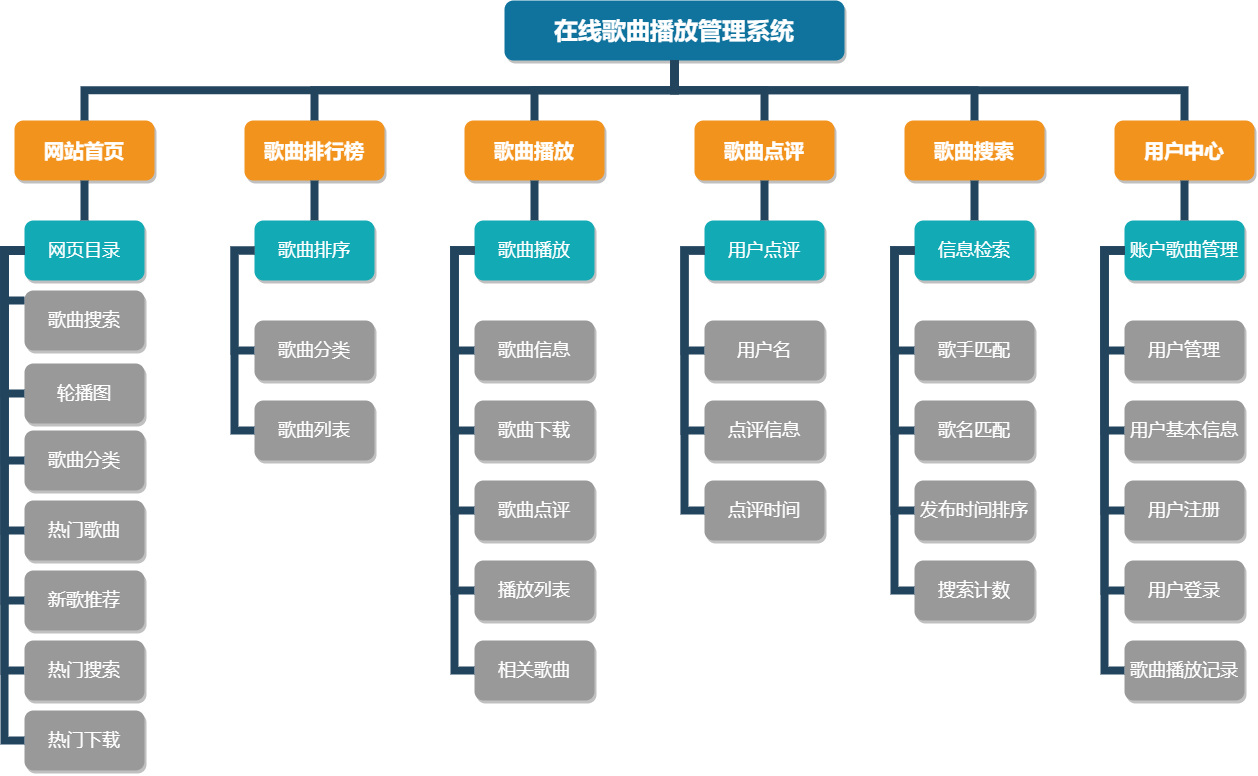
\includegraphics[width=10cm,height=11.59cm]{2.bmp}
    \caption{各节点的距离矢量表初始化}
\end{figure}
调用指令 gcc prog3.c node0.c node1.c node2.c node3.c -o test.exe 生成可执行文件并运行

\subsection{仿真结果}
\begin{figure}[ht]
    \centering
    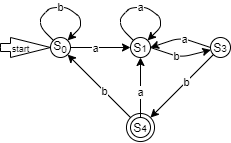
\includegraphics[width=11.59cm,height=5.73cm]{1.bmp}
    \caption{更新迭代后各结点最小矢量数组}
\end{figure}

\newpage
\section{五、总结与分析}
通过本次实验理解了Routing距离矢量表的更新过程,能够通过邻居结点的距离表信息更新自身路由表。
网络主机、路由器通过路由选择算法形成路由表,以确定发送分组的传输路径,而路由选择协议是
路由器用来完成路由表建立和路由信息更新的通信协议。
\end{document}